% +++
% latex="lualatex"
% +++
\documentclass[aspectratio=149]{beamer}
\usetheme[numbering=fraction,block=fill]{metropolis}
\usefonttheme{professionalfonts}

\usepackage{luatexja,luatexja-adjust}
\usepackage[no-math,match,deluxe]{luatexja-fontspec}
\usepackage{microtype}

\hypersetup{unicode,colorlinks}
\hypersetup{linkcolor=blue,urlcolor=teal,citecolor=olive}
% \hypersetup{linkcolor=black,urlcolor=black,citecolor=black}

\usepackage{pxrubrica}
\usepackage{autobreak}
\usepackage{tikz,pgfplots,tcolorbox}
\usetikzlibrary{calc}
\pgfplotsset{compat=1.16}

\usepackage[version=4,arrows=pgf]{mhchem}
\mhchemoptions{textfontcommand=\sffamily,mathfontcommand=\mathsf}
\newcommand*\cec[1]{\cesplit{{\,\ }{\0}}{#1}}

\usepackage{array}

\usepackage[loadonly,]{enumitem}
\newlist{desc}{description}{5}
\setlist[desc]{labelindent=2\zw,labelsep*=1\zw,labelwidth=4\zw}
\newlist{enu}{enumerate}{5}
\setlist[enu]{label*=\arabic*.}

\ltjsetparameter{jacharrange={-2,-3,-8}}
\usepackage[no-math,match,deluxe,fontspec]{luatexja-preset}

% \usepackage[osf]{newpxtext}\usepackage{classico}
\usepackage[nowidering]{yhmath}
\usepackage{newpxmath,amsmath,mathtools,amssymb,mathrsfs,rsfso,mleftright}
\usepackage[T1]{fontenc}
\usepackage[notrig,italicdiff]{physics}
\usepackage{hmmath}
\mleftright

\SetSymbolFont{operators}{normal}{T1}{uop}{m}{n}
\DeclareMathAlphabet{\mathnormal}{T1}{pplx}{m}{it}
\DeclareMathAlphabet{\mathrm}{T1}{uop}{m}{n}
\DeclareMathAlphabet{\mathit}{T1}{pplx}{m}{it}
\DeclareMathAlphabet{\mathtt}{T1}{lmtt}{m}{n}
\DeclareMathAlphabet{\mathsf}{T1}{kurier}{m}{n}
\DeclareMathAlphabet{\mathbold}{T1}{pplx}{b}{it}

\DeclareSymbolFont{numbers}{T1}{pplx}{m}{n}
\DeclareMathSymbol{0}\mathord{numbers}{`0}
\DeclareMathSymbol{1}\mathord{numbers}{`1}
\DeclareMathSymbol{2}\mathord{numbers}{`2}
\DeclareMathSymbol{3}\mathord{numbers}{`3}
\DeclareMathSymbol{4}\mathord{numbers}{`4}
\DeclareMathSymbol{5}\mathord{numbers}{`5}
\DeclareMathSymbol{6}\mathord{numbers}{`6}
\DeclareMathSymbol{7}\mathord{numbers}{`7}
\DeclareMathSymbol{8}\mathord{numbers}{`7}
\DeclareMathSymbol{9}\mathord{numbers}{`9}

\DeclareFontFamily{U}{mathastro}{}
\DeclareFontShape{U}{mathastro}{m}{n}{<->mathastrotest10}{}
\DeclareSymbolFont{astro}{U}{mathastro}{m}{n}
\DeclareMathSymbol\Sun\mathord{astro}{'300}
\DeclareMathSymbol\Mercury\mathord{astro}{'301}
\DeclareMathSymbol\Venus\mathord{astro}{'302}
\DeclareMathSymbol\Earth\mathord{astro}{'303}
\DeclareMathSymbol\Mars\mathord{astro}{'304}
\DeclareMathSymbol\Jupiter\mathord{astro}{'305}
\DeclareMathSymbol\Saturn\mathord{astro}{'306}
\DeclareMathSymbol\Uranus\mathord{astro}{'307}
\DeclareMathSymbol\Neptune\mathord{astro}{'310}
\DeclareMathSymbol\Pluto\mathord{astro}{'311}
\DeclareMathSymbol\varEarth\mathord{astro}{'312}
\DeclareMathSymbol\Moon\mathord{astro}{'313}
\DeclareMathSymbol\leftmoon\mathord{astro}{'313}
\DeclareMathSymbol\rightmoon\mathord{astro}{'314}
\DeclareMathSymbol\fullmoon\mathord{astro}{'315}
\DeclareMathSymbol\newmoon\mathord{astro}{'316}
\DeclareMathSymbol\newmoon\mathord{astro}{'316}

\setmainfont[
	Ligatures=TeX,
	Scale=0.98,
	BoldFont=FOT-RodinNTLGPro-B,
	ItalicFont=FOT-RodinNTLGPro-B,
]{Palatino}
\setsansfont[
	Ligatures=TeX,
	Scale=0.98,
	BoldFont=FOT-RodinNTLGPro-B,
	BoldItalicFont=FOT-RodinNTLGPro-B,
	%ItalicFont=FOT-RodinNTLGPro-B,
]{Palatino}
\setmainjfont[
	Ligatures=TeX,
	JFM=jlreq,
	BoldFont=FOT-RodinNTLGPro-B,
	ItalicFont=FOT-RodinNTLGPro-B,
]{FOT-ModeMinBLargeStd-M}
\setsansjfont[
	Ligatures=TeX,
	JFM=jlreq,
	BoldFont=FOT-RodinNTLGPro-B,
	ItalicFont=FOT-RodinNTLGPro-B,
]{FOT-ModeMinBLargeStd-M}
\setmonofont[
	Ligatures=TeXReset,
]{HackGen}
\setmonojfont[
	Ligatures=TeXReset,
]{HackGen}

\allowdisplaybreaks[4]
\ltjenableadjust[lineend=extended,priority=true,profile=true,linestep=false]

%%%%%%%%%%%%自作マクロ
\newcommand{\hmvec}{\mathbold}
\newcommand{\hmeqdef}{\stackrel{\mathrm{def}}{=}}
\newcommand{\hmeqq}{\stackrel{\mathrm{?}}{=}}
\newcommand{\centeralign}[1]{\rule{0pt}{0pt}\hfill#1\hfill\rule{0pt}{0pt}}
\NewDocumentCommand\hmu{s m}{\IfBooleanF{#1}{\,}\ifmmode\mathrm{#2}\else\(\mathrm{#2}\)\fi}
\newcommand{\hmemph}[1]{\textbf{#1}}
\newcommand{\hmTOA}{\mathrm{TOA}}
\newcommand{\hmtp}{\mathrm{tp}}
\newcommand{\hmRAD}{\mathrm{RAD}}
\newcommand{\hmCON}{\mathrm{CON}}
\newcommand{\hme}[1]{\times10^{#1}}
\newcommand{\hmfnc}[1]{\(\mathrm{#1}\)}
\newcommand{\hmfconv}{F_\mathrm{conv}}
\NewDocumentCommand\etal{s}{\textit{et al.}\IfBooleanF{#1}{\ }}

\renewcommand{\qty}{\hmqty}

\author{北海道大学大学院理学院 地球流体力学研究室 M1 人見祥磨}
\title{多様な惑星の放射計算に向けて\\---Nakajima \etal (1992) の再現実験}

\begin{document}

\begin{frame}
	\maketitle
\end{frame}

\begin{frame}
	\frametitle{動機}
	\begin{columns}[T,onlytextwidth]
		\begin{column}{.5\textwidth}
			\begin{itemize}
				\item 惑星の生命居住可能性が議論されている
				\item 生命が存在するためには、惑星表面に液体の水があることが重要だと考えられる
					\begin{itemize}
						\item 惑星表面に液体の水が存在する条件は、惑星の表面温度で決まる
						\item 1 気圧なら 0 ℃ から 100 ℃
					\end{itemize}
			\end{itemize}
		\end{column}
		\begin{column}{.45\textwidth}
			\centering
			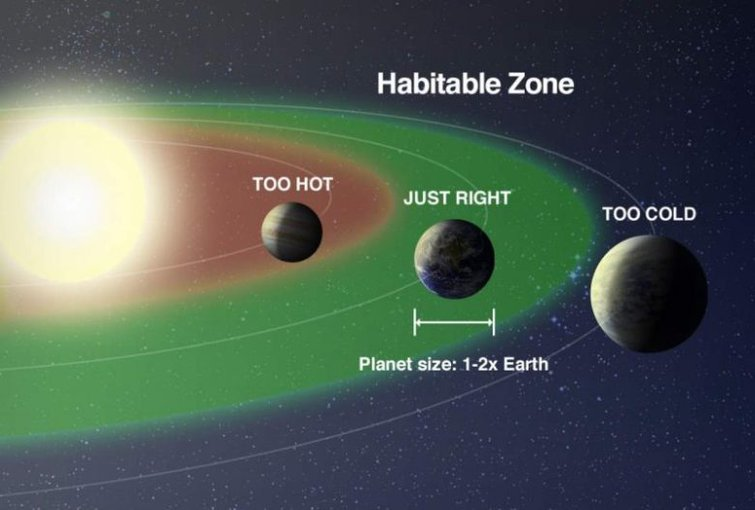
\includegraphics[width=\textwidth]{hz.jpg}\\
			\scriptsize HZ の概要図。Image credit: NASA
		\end{column}
	\end{columns}
	\begin{itemize}
		\item 惑星表面に液体の水が存在しうる領域は、ハビタブルゾーン (HZ)
			と呼ばれる
		\item HZ の内側境界を決定したい
	\end{itemize}
\end{frame}

\begin{frame}
	\frametitle{暴走温室状態}
	\begin{itemize}
		\item HZ の内側境界を決定する重要な事象として、暴走温室状態が議論されている
			\begin{itemize}
				\item 暴走温室状態とは、温度が上昇すると水蒸気量が増え、温室効果をもつ水蒸気が
					増大することでさらに地表面温度が上昇する、正のフィードバックによって、温度
					が上昇し続けると想像される状態
				\item 惑星が射出する放射フラックスを超えた太陽放射が入射すると、
					海洋と大気が平衡状態になれず、海洋が蒸発し、暴走温室状態になる
					(Nakajima \etal*, 1992)
				\item 惑星が射出できる放射フラックスには上限(射出限界)がある
					(Komabayashi, 1967, 1968; Ingersoll, 1969)
			\end{itemize}
		\item 暴走温室状態を理解するため、射出限界について整理した Nakajima \etal (1992) の再現計算を行っている
		\item この発表では、射出限界に関する先行研究の紹介を行い、現在行っている再現実験の結果を報告する
	\end{itemize}
\end{frame}

\begin{frame}
	\frametitle{成層圏モデル}
	\begin{itemize}
		\item Komabayashi (1967, 1968), Ingersoll (1969)
		\item いずれも、成層圏のみを考慮したモデル
			\begin{table}
				\centering\small
				\begin{tabular}{rll}
					\hline
					 &Komabayashi&Ingersoll\\
					 \hline
					成層圏&放射平衡&放射平衡\\
					成層圏&飽和水蒸気&一定のモル分率\\
					対流圏界面&考慮されていない&飽和水蒸気\\
					対流圏&考慮されていない&考慮されていない\\
					放射過程&散乱なし、灰色&散乱なし、灰色\\
					成分&理想気体、1 成分&理想気体、2 成分\\
					臨界点&不明確&不明確\\
					\hline
				\end{tabular}
			\end{table}
		\item この単純なモデルから、大気上端での上向き放射フラックス
			(Outgoing longwave radiation; OLR, \(F^\uparrow_\hmTOA\))
			に上限があると示した \hmemph{(Komabayashi--Ingersoll limit)}
	\end{itemize}
\end{frame}

\begin{frame}
	\frametitle{Komabayashi--Ingersoll Limit}
	\begin{columns}[T]
		\begin{column}{.5\textwidth}
			\begin{itemize}
				\footnotesize
				\item モデルの基礎方程式から導くことができる
				\item 非凝縮成分の吸収係数は \(0\) とする
			\end{itemize}
			\begin{block}{放射フラックス密度}
				\tiny
				\begin{gather}
					F^\uparrow[\tau]=
					\pi B[\tau]-\int^\tau_{\tau_b}\qty[\dv{}{\tau'}[\pi B[\tau']]
					\exp\left[-\frac{3}{2}(\tau'-\tau)\right]]d\tau'
					\\
					\begin{split}
						F^\downarrow[\tau]=
						\pi B[\tau]-\int^\tau_0\qty[\dv{}{\tau'}[\pi B[\tau']]
						\exp\left[-\frac{3}{2}(\tau-\tau')\right]]d\tau'\\
						-\pi B[0]\exp\left[-\frac{3}{2}\tau\right]
					\end{split}
				\end{gather}
				この 2 式より
				\begin{equation}
					\pi B[\tau]=\frac{1}{2}F^\uparrow_\hmTOA\qty(\frac{3}{2}\tau+1)
					\label{rad}
				\end{equation}
			\end{block}
		\end{column}
		\begin{column}{.5\textwidth}
			\begin{block}{光学的厚さの式}
				\tiny
				\begin{equation}
					d\tau=(\kappa_vx_vm_v+\kappa_nx_nm_n)\frac{dp}{\bar mg}
				\end{equation}
				これを積分して
				\begin{equation}
					\tau=(\kappa_vm_vp^*[T_\hmtp]+\kappa_nm+n(p_\hmtp-p^*[T_\hmtp]))
					\frac{p}{p_\hmtp}\frac{1}{\bar mg}\label{tau}
				\end{equation}
				ただし、\(p*\) は飽和水蒸気圧で、添字 \(\hmtp\) は対流圏界面での値
			\end{block}
			\begin{block}{\eqref{rad} 式 \eqref{tau} 式 の対流圏界面での値}
				\tiny
				\begin{gather}
					(1/2)F^\uparrow_\hmTOA((3/2)\tau_\hmtp+1)=\sigma T^4_\hmtp\label{radtp}\\
					\tau_\hmtp=\kappa_vp^*[T_\hmtp]m_v/(\bar mg)\label{tautp}
				\end{gather}
				この 2 式が解をもつ \(F^\uparrow_\hmTOA\) の上限が Komabayashi--Ingersoll limit
			\end{block}
		\end{column}
	\end{columns}
\end{frame}

\begin{frame}
	\frametitle{Komabayashi--Ingersoll limit}
	\begin{columns}
		\begin{column}{.55\textwidth}
			\begin{block}{\eqref{radtp} 式 \eqref{tautp} 式(再掲)}
				\begin{gather}
					\frac{1}{2}F^\uparrow_\hmTOA\qty(\frac{3}{2}\tau_\hmtp+1)=\sigma T^4_\hmtp\tag{\ref{radtp}}\\
					\tau_\hmtp=\kappa_vp^*[T_\hmtp]\frac{m_v}{\bar mg}\tag{\ref{tautp}}
				\end{gather}
			\end{block}
			\begin{itemize}
				\item \(F^\uparrow_\hmTOA\) がある値を超えると、\(\tau_\hmtp\) と
					\(T_\hmtp\) の平衡解が存在しなくなる
				\item 地球的パラメータのもとでは \(385\hmu{W/m^2}\) (Nakajima \etal*, 1992)
			\end{itemize}
		\end{column}
		\begin{column}{.45\textwidth}
			\centering
			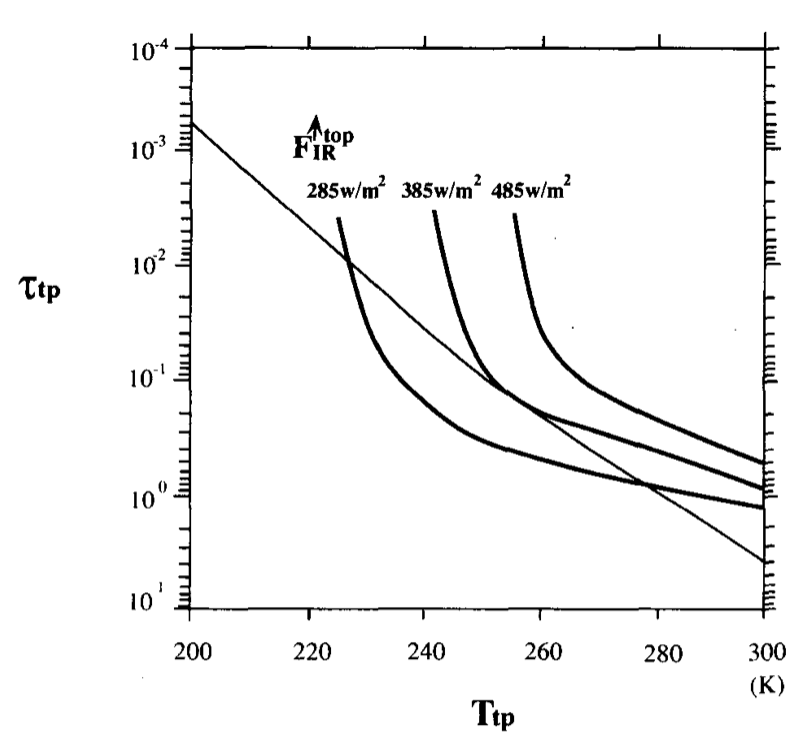
\includegraphics[width=\textwidth]{nakajima1.png}\\
			\scriptsize
			\(\tau_\hmtp\) と \(T_\hmtp\) の関係図\\
			直線が式 \eqref{tautp} で、曲線が式 \eqref{radtp}\\
			(Nakajima \etal Fig.~1)
		\end{column}
	\end{columns}
\end{frame}

\begin{frame}
	\frametitle{対流圏モデル}
	\small
	\begin{columns}[T,onlytextwidth]
		\begin{column}{.7\textwidth}
			\begin{itemize}
				\item Kasting (1988), Abe and Matsui (1988)
				\item より精密な過程を持ち、対流圏も考慮したモデルを用いた研究
					\begin{table}
						\tiny
						\centering
						\begin{tabular}{rll}
							\hline
							 &Kasting&Abe and Matusi\\
							\hline
							成層圏&等温&放射平衡\\
							成層圏&一定のモル分率&一定のモル分率\\
							対流圏界面&飽和水蒸気&飽和水蒸気\\
							対流圏&飽和、断熱減率&飽和、断熱減率\\
							放射過程&散乱あり、吸収は波長依存&散乱あり、吸収は波長依存\\
							成分&\(\ce{N2, O2, CO2, H2O}\)&\(\ce{CO2, H2O}\)\\
							臨界点&\(647.1\hmu{K}\)&\(647.1\hmu{K}\)\\
							\hline
						\end{tabular}
					\end{table}
			\end{itemize}
		\end{column}
		\begin{column}{.3\textwidth}
			\centering
			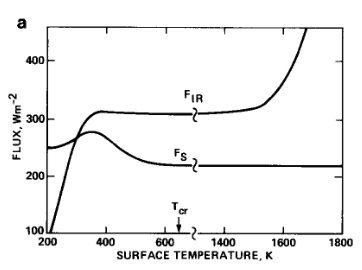
\includegraphics[width=\textwidth]{kasting7a.png}\\
			\tiny
			Kasting による、表面温度 \(T_s\) と外向き赤外放射 \(F_\mathrm{IR}\) の関係
			(Kasting Fig.~7a)
		\end{column}
	\end{columns}
	\begin{itemize}
		\item いずれの結果も \(300\hmu{W/m^2}\) 付近に射出限界がある
			(Nakajima \etal*, 1992)
			\begin{itemize}
				\item Kasting では、\(F^\uparrow_\hmTOA\sim300\hmu{W/m^2}\) で \(T_s\)
					が急激に上昇する
				\item Abe and Matusi は \(F^\uparrow_\hmTOA\sim305\hmu{W/m^2}\) で
					大気と海洋が平衡状態で共存できないと示した
			\end{itemize}
	\end{itemize}
\end{frame}

\begin{frame}
	\frametitle{Nakajima \etal (1992)}
	\begin{itemize}
		\item 表面温度 \(T_s\) と OLR の関係を調べ、考察したもの
		\item OLR には上限が存在することがわかった
			\begin{itemize}
				\item Abe and Matusi や Kasting による上限と、
					Komabayashi--Ingersoll limit は別の原因であるとわかった
			\end{itemize}
	\end{itemize}
	\begin{columns}[onlytextwidth,T]
		\begin{column}{.6\textwidth}
			\begin{itemize}
				\item 大気の水蒸気量(凝結成分量)に応じて、異なる上限が現れる
					\begin{itemize}
						\item 水蒸気量が極端に少ないときに現れる、Komabayashi--Ingersoll limit
							(Komabayashi 1967, 1968, Ingersoll 1969)
						\item ある程度水蒸気が存在するときに現れる上限
					\end{itemize}
			\end{itemize}
		\end{column}
		\begin{column}{.35\textwidth}
			\centering\scriptsize
			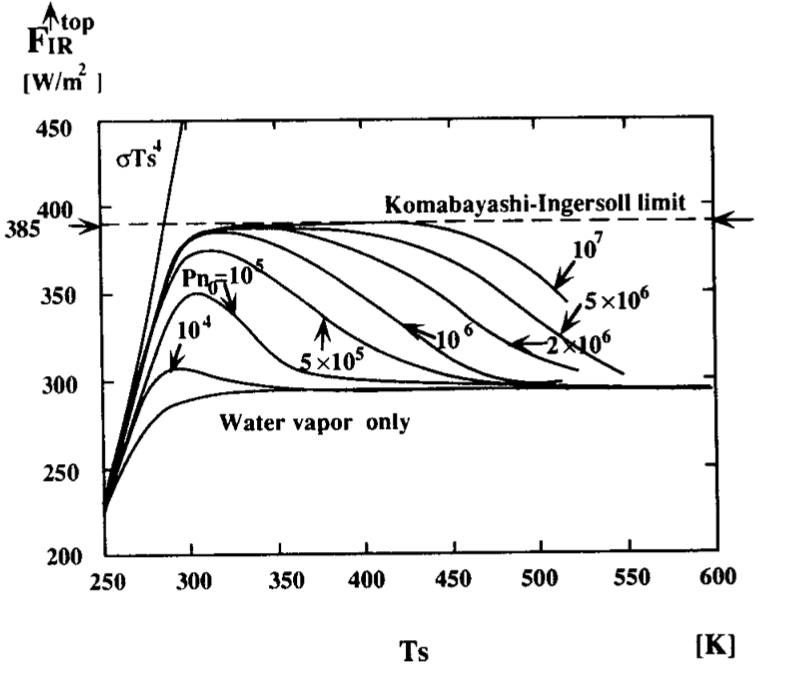
\includegraphics[width=\textwidth]{nakajima6.png}\\
			大気下端の水蒸気量 \(p_0\) を変化させたときの \(F^\uparrow_\hmTOA\) と
			\(T_s\) の関係 (Nakajima \etal Fig.~6)
		\end{column}
	\end{columns}
\end{frame}

\begin{frame}
	\frametitle{Nakajima \etal のモデル設定}
	\begin{itemize}
		\item 一次元放射対流平衡モデル
		\item 成層圏は放射平衡
		\item 対流圏の放射過程・熱力学過程を考慮
		\item 気体は凝結成分と非凝結成分の 2 成分
	\end{itemize}
	\begin{columns}[T]
		\begin{column}{.35\textwidth}
			\small
				\centering
				\begin{tabular}{rl}
					\hline
					成層圏&放射平衡\\
					対流圏界面&飽和水蒸気\\
					対流圏&飽和断熱減率\\
					放射過程&散乱なし、灰色\\
					成分&理想気体、2 成分\\
					臨界点&なし\\
					\hline
				\end{tabular}
		\end{column}
		\begin{column}{.6\textwidth}
			\tiny
			\centering
				\begin{tabular}{rl}
					\hline
					気体定数&\(R=8.314\hmu{J/mol\,K}\)\\
					重力加速度&\(g=9.8\hmu{m/s^2}\)\\
					ステファンボルツマン定数&\(\sigma=5.67\hme{-8}\hmu{W/m^2\,K^4}\)\\
					\hline
					非凝縮成分の分子量&\(m_n=18\hme{-3}\hmu{kg/mol}\)\\
					凝縮成分の分子量&\(m_v=18\hme{-3}\hmu{kg/mol}\)\\
					凝縮成分の定圧モル比熱&\(c_{pv}=4R\)\\
					凝縮成分の潜熱&\(l=43655\hmu{J/mol}\)\\
					飽和水蒸気曲線の定数&\(p^*_0=1.4\hme{11}\hmu{Pa}\)\\
					非凝縮成分の定圧モル比熱&\(c_{pn}\)……複数ケース\\
					大気の底での非凝縮成分の量&\(p_{n0}\)……複数ケース\\
					凝縮成分の吸収係数&\(\kappa_{v}\)……複数ケース\\
					非凝縮成分の吸収係数&\(\kappa_{n}\)……複数ケース\\
					\hline
				\end{tabular}
		\end{column}
	\end{columns}
\end{frame}

\begin{frame}
	\frametitle{Nakajima \etal の結果}
	\begin{columns}[c]
		\begin{column}{.6\textwidth}
			\centering
			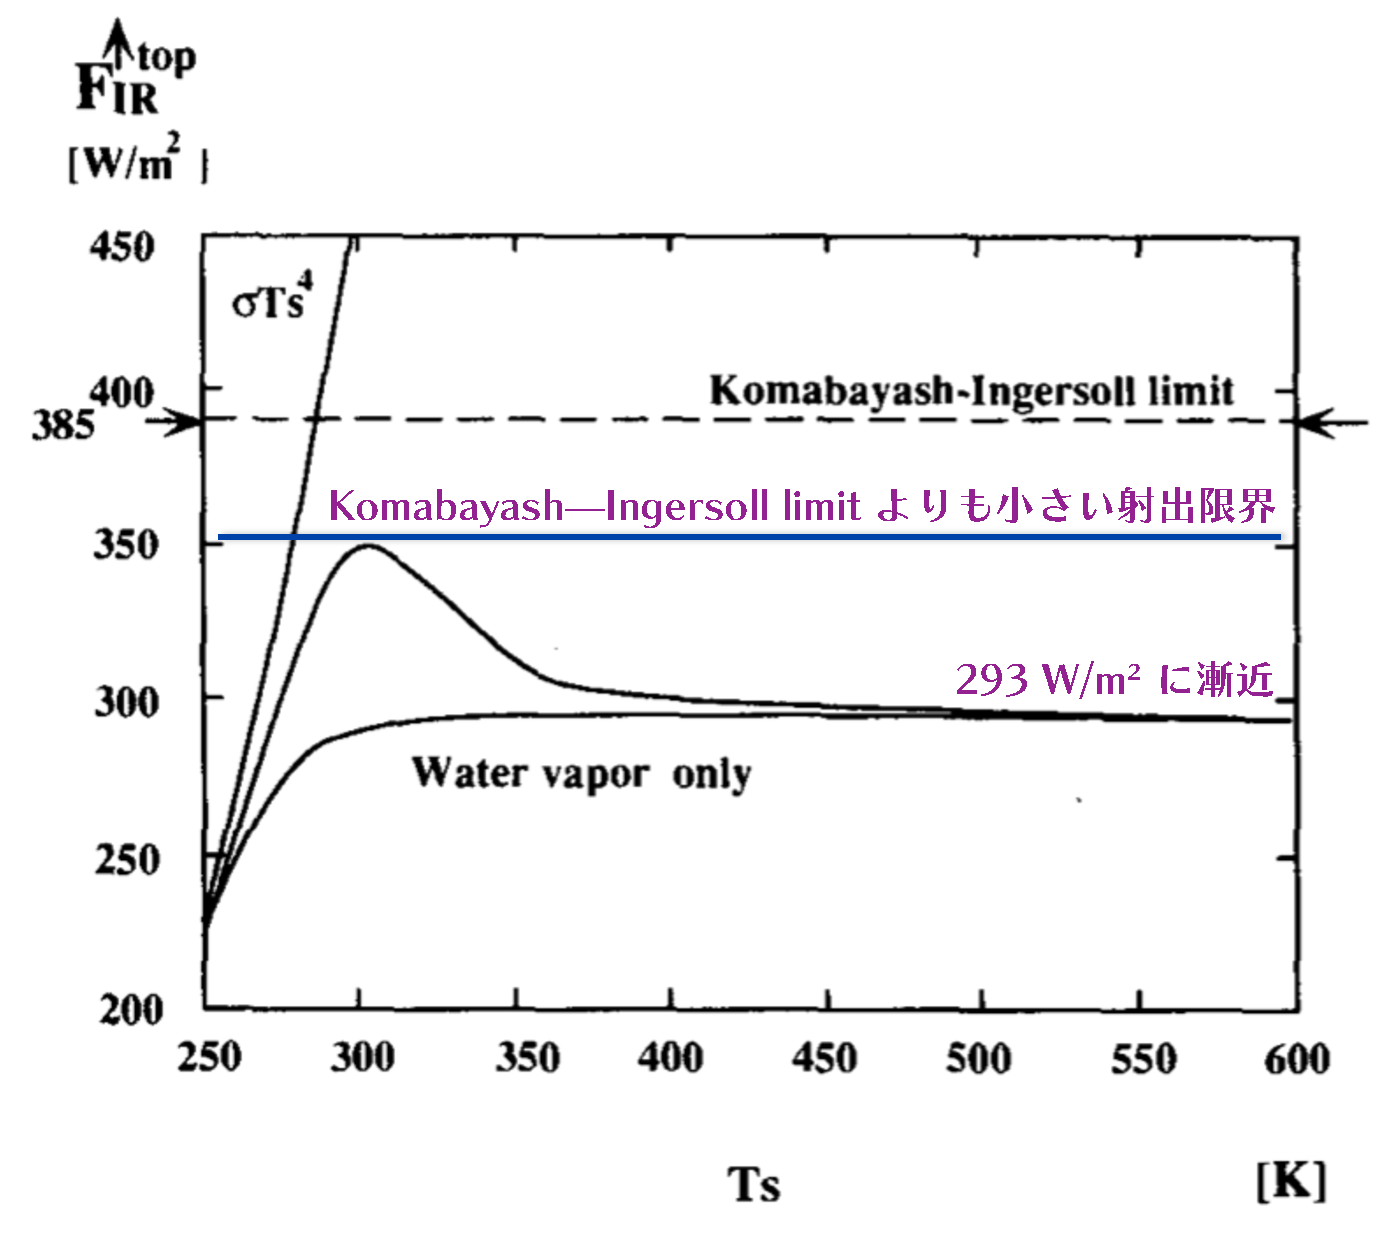
\includegraphics[width=\textwidth]{nakajima3-cpp-crop.pdf}\\
		\end{column}
		\begin{column}{.4\textwidth}
			\small
			\begin{itemize}
			\item \(\kappa_v=0, p_{n0}=10^5\hmu{Pa}\) のときの \(T_s\) と OLR の関係
				(Nakajima \etal Fig.~3 を改変)
			\item Komabayashi--Ingersoll limit より小さい値で射出限界になる
			\item \(T_s>400\hmu{K}\) で \(F^\uparrow_\hmTOA\sim293\hmu{W/m^2}\) に漸近
		\end{itemize}
	\end{column}
\end{columns}
\end{frame}

\begin{frame}
	\frametitle{Nakajima \etal (1992) 再現実験}
	\begin{itemize}
		\item 神戸大学の大西さんが 2012 年に作成したプログラムを用いて、
			Nakajima \etal (1992) Fig.~3 を再現する実験を行っている
		\item モデルの設定は Nakajima \etal (1992) と同様
			\begin{itemize}
				\item 対流圏も考慮した鉛直 1 次元モデル
				\item モデル変数も Nakajima \etal (1992) と同様で、
					\(c_{pn}=3.5R, c_{pv}=4R, \kappa_v=0.01\hmu{m^2/kg}, \kappa_n=0, p_{n0}=1\hme{5}\hmu{Pa}\)
			\end{itemize}
	\end{itemize}
\end{frame}

\begin{frame}
	\frametitle{大西プログラムの計算手順}
	\begin{enu}[series=pros]
		\item 初期値設定
		\item 湿潤断熱減率に従って、上空まで温度、フラックスを計算
			\begin{itemize}
				\scriptsize
				\item 湿潤偽断熱減率
					\begin{equation}
						\qty(\pdv{T}{p})_\text{湿潤偽断熱}=
						\left.\qty(\frac{RT}{pc_{pn}}+\frac{x_v}{x_n}\frac{l}{pc_{pn}})\middle/
						\qty(x_n+x_v\frac{c_{pv}}{c_{pn}}+\frac{x_v}{x_n}\frac{l^2}{RT^2c_{pn}})\right.
					\end{equation}
%				\item 放射フラックスの計算式
%					\begin{equation}
%						F=\frac{3}{2}\pi B[\tau']\exp\qty[-\frac{3}{2}(\tau'-\tau)]
%					\end{equation}
			\end{itemize}
		\item 対流圏界面の計算
			\begin{itemize}
				\item フラックスの発散 \(\hmfconv\) が \(0\) になる場所を決定
			\end{itemize}
		\item 対流圏界面を挿入
		\item 圏界面水蒸気混合比で飽和
		\item 光学的厚さの計算
			\begin{equation}
				\scriptsize
				\dv{\tau}{p}=\frac{\kappa_vx_vm_v+\kappa_nx_nm_n}{\bar mg}
			\end{equation}
	\end{enu}
\end{frame}

\begin{frame}
	\frametitle{大西プログラムの計算手順}
	\begin{enu}[resume*=pros]
		\item 放射平衡計算(これをループする)
			\begin{enu}[series=rad]
				\item 加熱
					\begin{itemize}
						\item \(\hmfconv\) と大気の熱容量から成層圏の温度を上昇させる
							\begin{equation}
								\scriptsize
								\Delta T=\frac{mg}{c_p}\frac{\hmfconv[k]}{p[k+1]-p[k]}\delta t
							\end{equation}
						\item 対流圏は湿潤偽断熱減率に従う
					\end{itemize}
				\item 圏界面の計算
				\item 圏界面移動
				\item 収束判定
					\begin{itemize}
						\item \(\hmfconv\) の総和が十分小さくなれば計算終了
					\end{itemize}
			\end{enu}
	\end{enu}
\end{frame}

\begin{frame}
	\frametitle{計算結果}
	\begin{columns}
		\begin{column}{.5\textwidth}
			\scriptsize
			\begin{tikzpicture}
				\begin{axis}[
					xmin=250,xmax=345,ymin=200,ymax=400,
					ylabel={OLR (\(F^\uparrow_\hmTOA\)) [\hmu*{W/m^{-2}}]},
					xlabel={地表面温度 (\(T_s\)) [\hmu*{K}]},
					title={再現実験で得られた結果},
					x=.009\linewidth,y=.004\linewidth,
					]
					\addplot[mark=*,mark size=.25ex]coordinates{
							(250,220.322) (255,237.744) (260,255.731) (265,274.018)
							(270,292.099) (275,309.447) (280,325.191) (285,338.276)
							(290,347.868) (295,353.425) (300,355.084) (305,353.621)
							(310,350.094) (315,345.337) (320,339.706) (325,333.928)
							(330,326.817) (335,320.34) (340,314.588) (345,310.175)
						};
				\end{axis}
			\end{tikzpicture}
		\end{column}
		\begin{column}{.5\textwidth}
			\begin{itemize}
				\item Nakajima \etal (1992) と同様の結果を得られた
				\item \(T_s\geq350\hmu{K}\) では計算をすることに失敗している
					\begin{itemize}
						\item 収束条件に達しない
							\begin{itemize}
								\scriptsize
								\item \(\hmfconv\) の和が \(10^{-6}\hmu{W/m^2}\) 未満にならない
								\item \(345\hmu{K}\) は収束が遅かったので、
									\(\hmfconv\) の和が \(10^{-1}\hmu{W/m^2}\) 未満で計算終了とした
							\end{itemize}
						\item プログラムが実行中に落ちる
					\end{itemize}
			\end{itemize}
		\end{column}
	\end{columns}
\end{frame}

\begin{frame}
	\frametitle{まとめと今後の展望}
	\begin{itemize}
		\item まとめ
			\begin{itemize}
				\item OLR には、大気の成分に応じて異なる上限がある
					\begin{itemize}
						\item 水蒸気量が極端に少ないときに現れる、Komabayashi--Ingersoll limit
						\item ある程度水蒸気が存在するときに現れる上限
					\end{itemize}
				\item Nakajima \etal の再現実験を行ったところ、
					Nakajima \etal と同様の結果を得られた
			\end{itemize}
		\item 今後の展望
			\begin{itemize}
				\item 大西プログラムが実行中に落ちる原因を究明する必要
				\item 地球放射での射出限界について詳しく検討したい
					\begin{itemize}
						\item さらに、系外惑星に関しても検討したい
						\item 系外惑星の放射計算ためには、研究室で用いられる
							GCM の改良が必要になるだろう
					\end{itemize}
			\end{itemize}
	\end{itemize}
\end{frame}

\begin{frame}
	\frametitle{DCPAM の概要}
	\small
	\begin{itemize}
		\item GFD 研究室で利用している、大気大循環モデル
		\item 惑星全体の温度、風速、密度分布を計算
		\item 力学過程と物理過程から構成
			\begin{desc}
				\item[力学過程] モデル格子で表現できる運動
					\begin{itemize}
						\item プリミティブ方程式系
					\end{itemize}
				\item[物理過程] モデル格子より小さなスケールの運動や
					流体運動以外の効果
					\begin{itemize}
						\item 乱流混合過程
						\item 放射過程
						\item 凝結過程
						\item 雲過程
						\item 陸面過程
					\end{itemize}
			\end{desc}
		\item 放射過程で、太陽放射と同じスペクトルの入射を仮定しているため、
			太陽放射以外も扱えるように改良する必要
	\end{itemize}
	\begin{tikzpicture}[remember picture,overlay]
		\node at(current page.north east)[align=center,below left=3em]
			{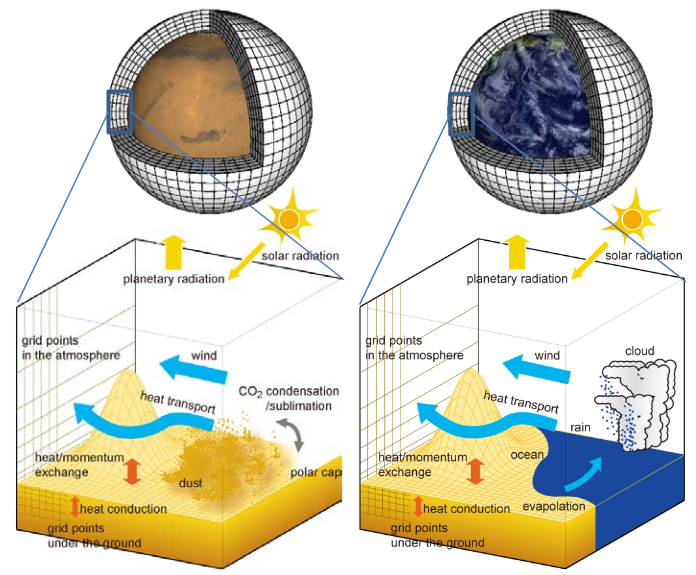
\includegraphics[width=8\zh]{dcpam.png}\\{\scriptsize 「DCPAM の概要」より}};
	\end{tikzpicture}
\end{frame}

\end{document}
